\documentclass[11pt]{beamer}
\usetheme{CambridgeUS}
\usepackage[utf8]{inputenc}
\usepackage[english]{babel}
\usepackage{amsmath}
\usepackage{mathtools, amsthm, amssymb, amsfonts}
\usepackage{graphicx}
\usepackage{tabularx}

\usepackage{tikzsymbols}
\usepackage{textcomp}
\usepackage{phaistos}
\usepackage{tikz}
\usetikzlibrary{arrows.meta,topaths}% <-- new
\tikzset{loop arrow/.style={% <-- new
    -{Stealth[length=8mm]}, draw=green!40!red,
    bend left=28}}

\newcommand{\tikzmark}[1]{\tikz[overlay,remember picture] \node (#1) {};}

\tikzset{square arrow/.style={
    to path={-- ++(0,-2.25)  -| (\tikztotarget) \tikztonodes},below,pos=3.75}}
\newcommand\myleaf{\mbox{\textleaf}}
\newcommand\mytree{\mbox{\PHplaneTree}}
\DeclareMathOperator*{\argmax}{arg\,max}

\renewcommand{\vec}[1]{\ushort{#1}}
\renewcommand{\vec}[1]{\mathbf{#1}}

\usepackage{bigints}





\author{F. Richter Mendoza}
\title{Updates}
%\setbeamercovered{transparent} 
%\setbeamertemplate{navigation symbols}{} 
%\logo{} 
%\institute{} 
%\date{} 
%\subject{} 
\begin{document}

%\begin{frame}
%\titlepage
%\end{frame}

%\begin{frame}
%\tableofcontents
%\end{frame}


\begin{frame}{}
 \emph{ ``Evolution is not to be understood as a series of tournaments for the occupation of a fixed set of enviromental niches... Instead evolution brings about a proliferation of niches... Each new bird or mammal provides a niche for one or more new kind of flea.''}
  \vskip5mm
  \hspace*\fill{\small--- Herbert Simon, The Sciences of the Artificial, 1969.}
\end{frame}

\begin{frame}
The aim of this project is to develop {\bf realistic stochastic models} and
{\bf reliable statistical inference methods} for species diversification.\pause \\ \vspace{1cm}
	
	To do that we mainly face two big challenges: 
\begin{columns}
\begin{column}{0.5\textwidth}


%\begin{itemize}
%\item Complexity
$\bullet$ Complexity
 \begin{figure}
                	%\vspace*{-1cm}
                    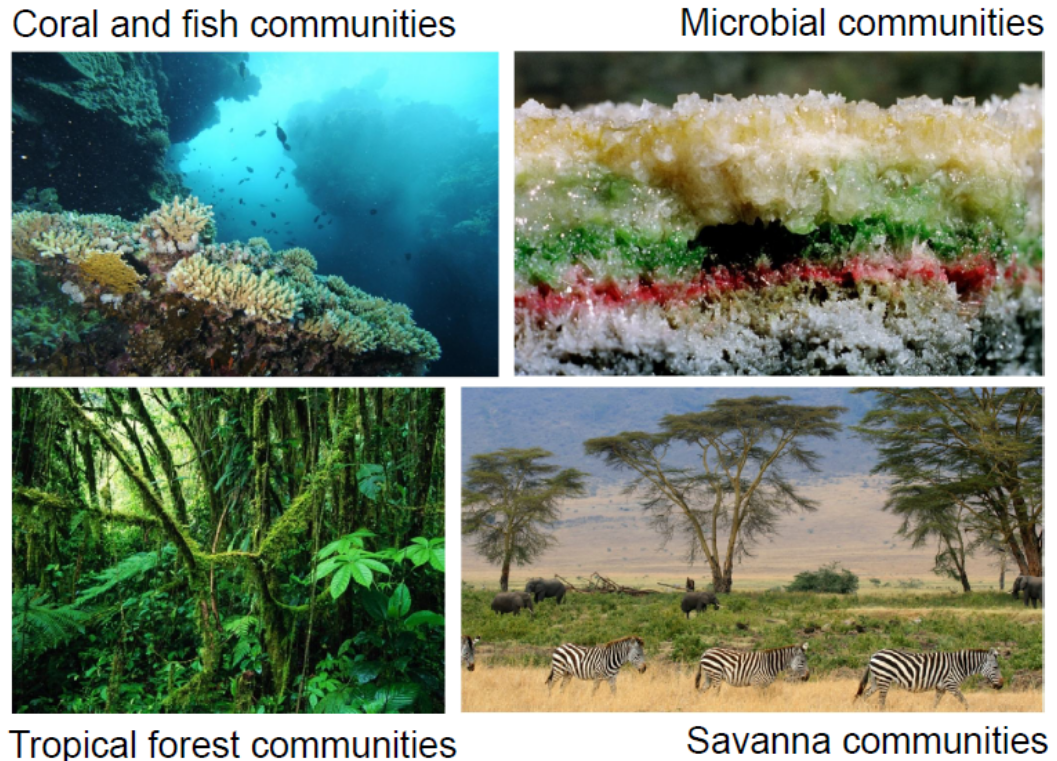
\includegraphics[width=0.61\linewidth]{figures/communities.png}
		\end{figure}
\end{column}
\begin{column}{0.5\textwidth}  %%<--- here
    %\begin{center}
     %\includegraphics[width=0.5\textwidth]{image1.jpg}
     %\end{center}
    % \item 
    $\bullet$  Incomplete information

      \begin{figure}
                    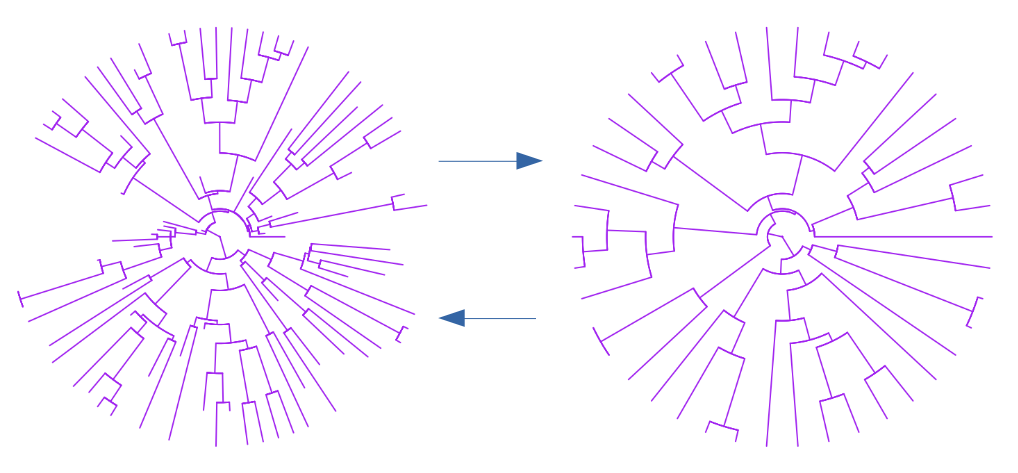
\includegraphics[width=0.85\linewidth]{figures/treesa.png}
                 
				\end{figure}
  %   \end{itemize}
\end{column}
\end{columns}






\end{frame}

\begin{frame}{Set up}
The phylogenetic tree is mathematically determined by

\begin{itemize}
	\item A set of branching times $\mathcal{T}$% = \{t_1,t_2,...,t_n\}$.
	\item The topology  $\Upsilon$.% = \{ \mathfrak{S}, \mathfrak{X} \}$.   
\end{itemize}

And its likelihood function is defined as 

	\begin{equation} L( Y | \Theta) = \displaystyle\prod_{i=1}^p \sigma_i e^{-\sigma_i t_i} \frac{\rho_{i}}{\sigma_i}  
 		\label{llik}
 		\end{equation}
 		
\end{frame}

\begin{frame}{Example: Diversity-dependence model}
For the simplest diversity-dependence model 

$$ \lambda_{i,j} = \lambda_0 - (\lambda_0 - \mu_0)\frac{n_i}{K}, \qquad \mu_n = \mu_0 $$ 

The MLE can be finded partially analiticaly and partially numerically. \pause First we consider $\sigma_i$ and $\rho_i$ 

$$ \sigma_i  = \sum_{j=1}^{N}  \lambda_0 - (\lambda_0 - \mu_0)\frac{n_i}{K} + \mu_0 
 		 = n_i(\lambda_0 + \mu_0) - n_i^2\beta_0 $$

where $ \beta_0=\left(\frac{\lambda_0-\mu_0}{K}\right)$, and

$$\rho_i = E_i(\lambda_0 - n_i\beta_0)+(1-E_i)\mu_0$$
\end{frame}

\begin{frame}

Firstly, after some algebra, we find a very nice analytical solution for the extinction rate parameter
\begin{equation}
\label{mu}
 \frac{\partial l(\lambda,\beta,\mu | Y)}{\partial \mu} = 0  \Leftrightarrow \hat{u}_0 = \frac{\displaystyle\sum_{i=1}^N (1-E)}{\displaystyle\sum_{i=1}^N(n_it_i)} 
\end{equation}
\pause
Moreover, with the other two equations, we have the following system
$$\begin{cases} \displaystyle\sum_{i=1}^N \frac{E_i}{\lambda-n_i\beta} = \displaystyle\sum_{i=1}^N n_i t_i \\ \displaystyle\sum_{i=1}^N \frac{E_in_i}{\lambda-n_i\beta} = \displaystyle\sum_{i=1}^N n^2_i t_i \end{cases}$$

\end{frame}

\begin{frame}

\begin{table}[h!]
{\tiny
\centering

\caption{MLE estimation of 100 simulations. Simulations and estimations are from the algorithm described above.}
\label{alg}
\begin{tabular}{cccc|ccc@{\hskip 0.2in}ccc@{\hskip 0.2in}ccc}
\hline
\multicolumn{4}{c}{Simulated Parameters} & \multicolumn{9}{c}{Estimated parameters (25th, 50th, 75th percentiles)} \\ \hline
$\lambda_0$    & $K$     & crown age    & $\mu$    &        & $\lambda_0$  &       &       & $\mu$   &      &       & $K$     &        \\
          &       &              &       & 025th  & 50th    & 75th  & 025th & 50th & 75th & 025th & 50th  & 75th   \\
          &       &              &       &        &         &       &       &      &      &       &       &        \\
0.8       & 40    & 5            & 0     & 0.71   & 0.87    & 1.04  & 0.00  & 0.00 & 0.00 & 31.20 & 39.09 & 440.16 \\
          &       &              & 0.1   & 0.76   & 0.92    & 1.11  & 0.07  & 0.10 & 0.13 & 22.23 & 32.65 & 65.39  \\
          &       &              & 0.2   & 0.80   & 0.96    & 1.28  & 0.13  & 0.19 & 0.26 & 12.74 & 31.76 & 83.12  \\
          &       &              & 0.4   & 1.05   & 1.23    & 1.55  & 0.27  & 0.36 & 0.44 & 7.00  & 17.61 & 30.58  \\
          &       &              &       &        &         &       &       &      &      &       &       &        \\
          &       & 10           & 0     & 0.68   & 0.79    & 0.87  & 0.00  & 0.00 & 0.00 & 39.63 & 40.98 & 43.92  \\
          &       &              & 0.1   & 0.71   & 0.86    & 0.98  & 0.09  & 0.10 & 0.12 & 37.11 & 39.52 & 42.01  \\
          &       &              & 0.2   & 0.78   & 0.91    & 1.05  & 0.18  & 0.20 & 0.23 & 34.08 & 38.13 & 43.32  \\
          &       &              & 0.4   & 0.87   & 1.01    & 1.20  & 0.37  & 0.41 & 0.46 & 18.32 & 30.13 & 42.13  \\
          &       &              &       &        &         &       &       &      &      &       &       &        \\
          &       & 15           & 0     & 0.69   & 0.77    & 0.87  & 0.00  & 0.00 & 0.00 & 39.58 & 40.00 & 41.03  \\
          &       &              & 0.1   & 0.72   & 0.80    & 0.91  & 0.09  & 0.10 & 0.11 & 38.72 & 39.89 & 40.98  \\
          &       &              & 0.2   & 0.78   & 0.84    & 0.96  & 0.18  & 0.20 & 0.22 & 38.29 & 40.25 & 41.93  \\
          &       &              & 0.4   & 0.79   & 0.90    & 1.00  & 0.38  & 0.40 & 0.43 & 31.40 & 37.38 & 43.89 
\end{tabular}
}
\end{table}

\end{frame}

\begin{frame}


\begin{table}[h!]
{\tiny
\centering

\caption{MLE estimation of 100 simulations. Simulations are from the 'DDD' package and estimation from p1 algorithm.}
\label{ddd}
\begin{tabular}{cccc|ccc@{\hskip 0.2in}ccc@{\hskip 0.2in}ccc}
\hline
\multicolumn{4}{c}{Simulated Parameters} & \multicolumn{9}{c}{Estimated parameters (25th, 50th, 75th percentiles)} \\ \hline
     %   &       &              &        &         &       &       &        &       &       &       &       &       \\
$\lambda_0$     & $K$     & crown age    & $\mu$     &   &  $\lambda_0$     &       &      &  $\mu$     &       &      &  $K$     &       \\
           &       &              &        & 025th   & 50th  & 75th  & 025th  & 50th  & 75th  & 025th & 50th  & 75th  \\
            &       &              &       &        &         &       &       &      &      &       &       &        \\ 
0.8        & 40    & 5            & 0      & 0.74    & 0.91  & 1.11  & 0.00   & 0.00  & 0.00  & 34.84 & 41.04 & 59.34 \\
           &       &              & 0.1    & 0.94    & 1.15  & 1.28  & 0.08   & 0.11  & 0.14  & 26.57 & 32.55 & 39.98 \\
           &       &              & 0.2    & 1.03    & 1.22  & 1.46  & 0.17   & 0.21  & 0.29  & 17.06 & 27.85 & 37.47 \\
           &       &              & 0.4    & 1.13    & 1.43  & 1.67  & 0.33   & 0.42  & 0.52  & 9.40  & 17.52 & 27.29 \\
           &       &              &        &         &       &       &        &       &       &       &       &       \\
           &       & 10           & 0      & 0.75    & 0.87  & 0.98  & 0.00   & 0.00  & 0.00  & 38.55 & 39.33 & 40.35 \\
           &       &              & 0.1    & 0.78    & 0.90  & 1.05  & 0.09   & 0.10  & 0.12  & 37.09 & 38.55 & 40.33 \\
           &       &              & 0.2    & 0.86    & 0.96  & 1.08  & 0.19   & 0.21  & 0.23  & 34.47 & 37.45 & 40.38 \\
           &       &              & 0.4    & 0.96    & 1.11  & 1.22  & 0.38   & 0.42  & 0.45  & 28.11 & 33.88 & 40.41 \\
           &       &              &        &         &       &       &        &       &       &       &       &       \\
           &       & 15           & 0      & 0.74    & 0.83  & 0.96  & 0.00   & 0.00  & 0.00  & 38.57 & 39.05 & 40.00 \\
           &       &              & 0.1    & 0.80    & 0.88  & 0.99  & 0.09   & 0.11  & 0.12  & 37.57 & 38.67 & 39.57 \\
           &       &              & 0.2    & 0.88    & 0.95  & 1.05  & 0.20   & 0.21  & 0.22  & 36.98 & 38.58 & 40.07 \\
           &       &              & 0.4    & 0.92    & 1.03  & 1.14  & 0.38   & 0.41  & 0.44  & 34.02 & 37.45 & 41.96
\end{tabular}
}
\end{table}



\end{frame}

\begin{frame}
 \begin{figure}[h]
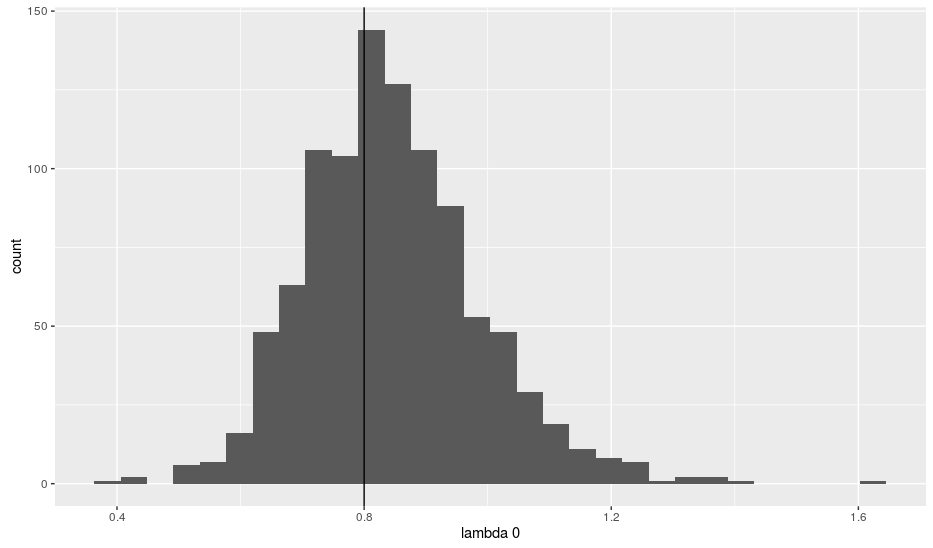
\includegraphics[width=.35\textwidth]{lambda.png}
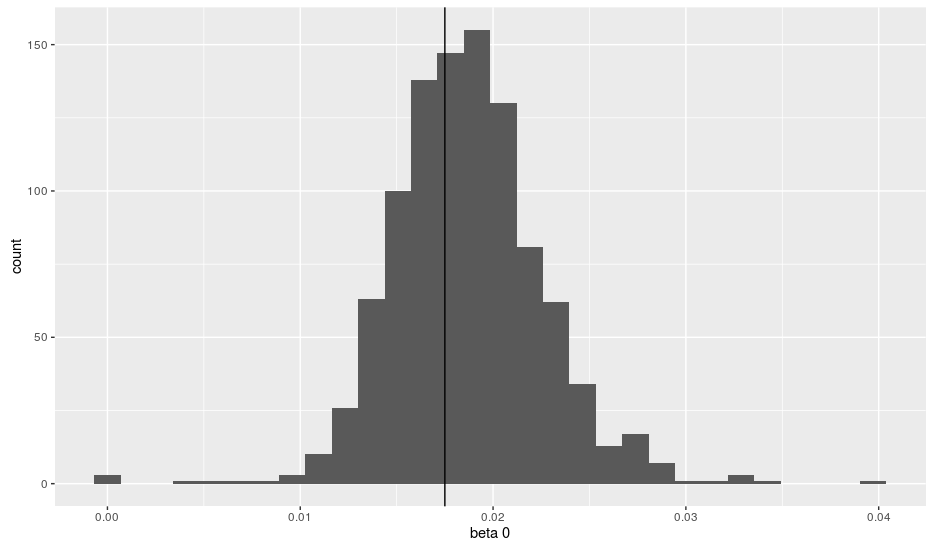
\includegraphics[width=.35\textwidth]{beta.png}\\
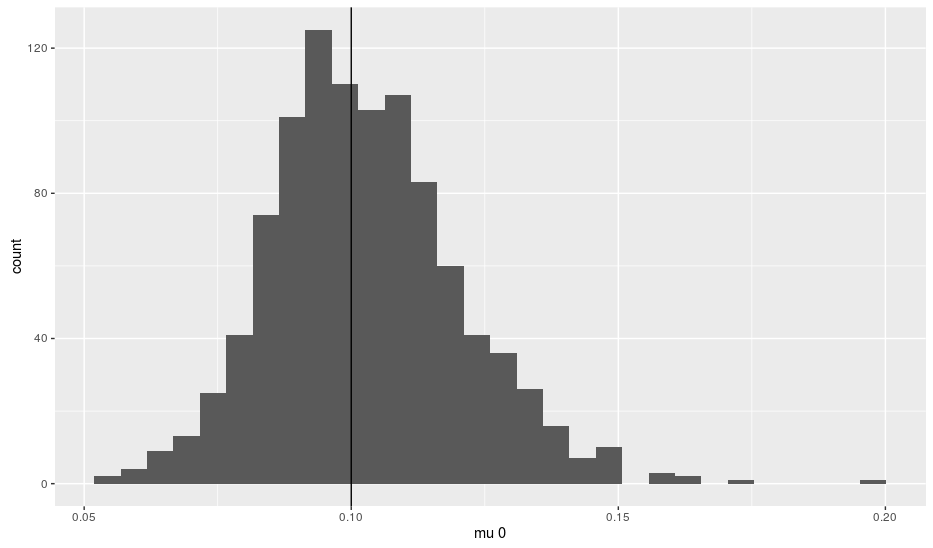
\includegraphics[width=.35\textwidth]{mu.png}
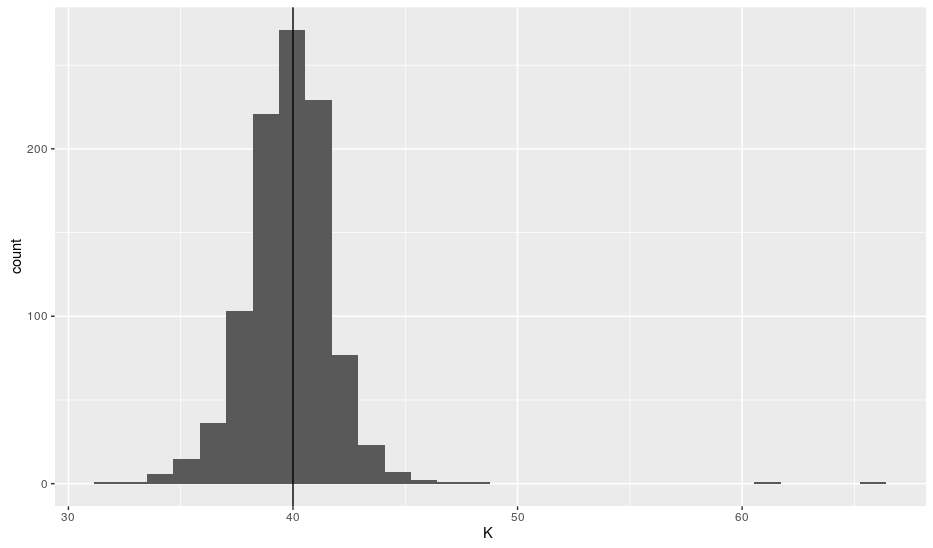
\includegraphics[width=.35\textwidth]{K.png}
%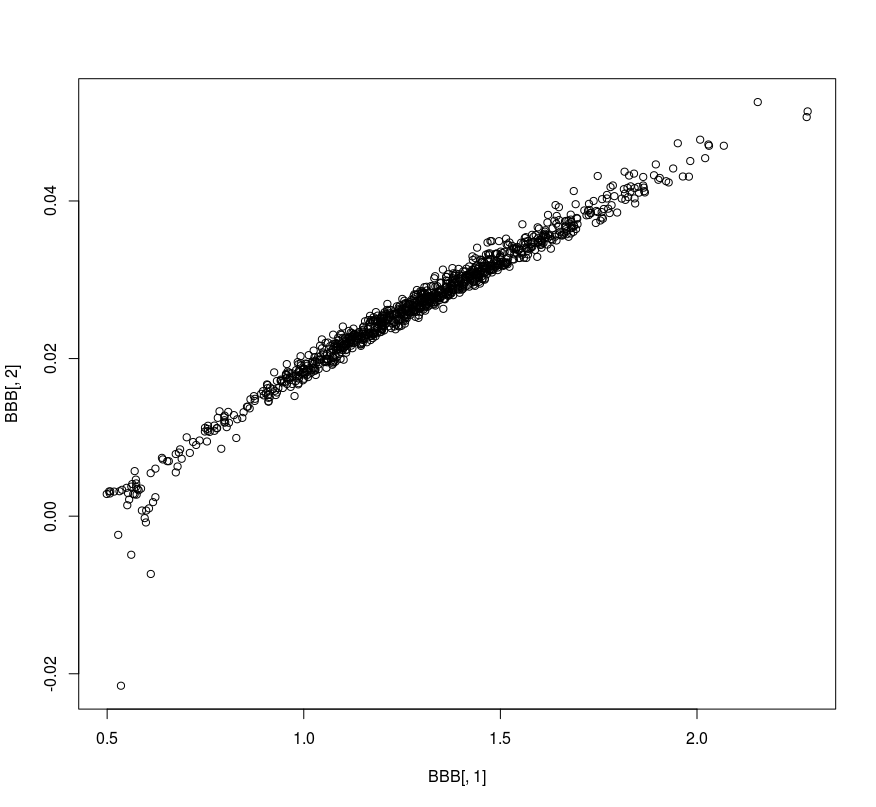
\includegraphics[width=.5\textwidth]{bolh.png}
%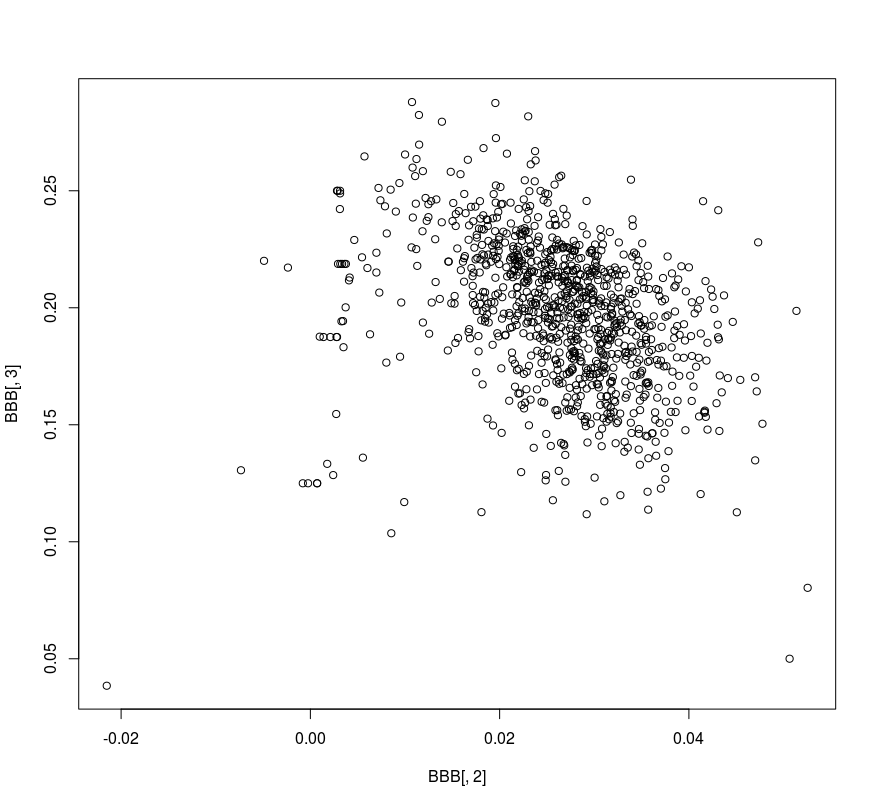
\includegraphics[width=.5\textwidth]{b0mh.png}
\label{hists}
\caption{Estimations over 1000 simulations of the diversity-dependence process with true values $\lambda_ = 0.8, \beta_0 = 0.0175, \mu_0 = 0.1, K=40$ and crown time $=15$. The black vertical lines shows the real values.}
\end{figure}
\end{frame}

\begin{frame}{Developing statistical SDE inference procedures}

The likelihood is only {\bf explicit} given the {\bf full} phylogenetic history S:

$$ S = (D,M), $$

where $M$ is missing data (extinct species, incomplete fossil record, ...). 

\begin{block}{EM algorithm}

For unimodal likelihoods, its unique maximum can be found by maximizing iteratively 
$$ Q(\theta | \theta^{(i-1)}) = E[l_{D,M}(\theta) | D, \theta^{(i-1)} ] $$ 
\end{block}


\end{frame}

\begin{frame}{MCEM}
\[
Q(\theta | \textcolor{red}{\theta_{(i\tikzmark{a})}})% <-- changed
    = \smashoperator[r]{\bigint_{\{\small
                           \Springtree, \Autumntree, \Summertree, \dots \}}
                        }
    \log L(\theta|\Wintertree) \mathrm{d}\Wintertree \longrightarrow
           \textcolor{red}{\theta_{(i\tikzmark{b}+1)}}% <-- changed
    = \displaystyle\argmax_{\theta} Q\left(\theta | \theta_{(i)}\right)
\]
\end{frame}
\end{document}